\section{Forces in Equilibrium}

\begin{multicols}{2}


\section*{Effect of Turning Forces}


\subsection{Ruler Balance}

\begin{center}
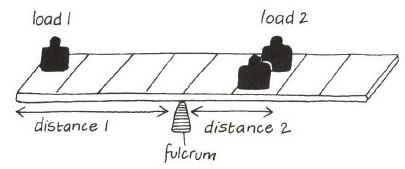
\includegraphics[width=0.45\textwidth]{./img/vso/lever-balance.jpg}
\end{center}

\begin{description*}
%\item[Subtopic:]{}
\item[Materials:]{Ruler, small weights (e.g. coins), fulcrum (e.g. knife or ruler)}
%\item[Setup:]{}
\item[Procedure:]{Balance the ruler on the fulcrum (15 cm mark). Add coins to either side at different distances in order to keep the ruler balanced. Repeat by starting the ruler at the 10 cm or 20 cm marks.}
%\item[Hazards:]{}
%\item[Questions:]{}
\item[Observations:]{Larger loads require shorter distances to balance, while smaller loads require longer distances from the fulcrum.}
\item[Theory:]{$\text{Moment} = \text{Force} \times \text{Lever arm}$. In order to balance, the moments on either side of the pivot must be equal. When the lever arm of one side is larger, more weight must be added to the shorter side to balance.}
%\item[Applications:]{}
%\item[Notes:]{}
\end{description*}

%\begin{description*}
%%\item[Subtopic:]{}
%\item[Materials:]{2 rulers, bottle caps, toilet paper tube, tape, cardboard}
%\item[Setup:]{Make a knife edge by fixing a ruler vertically in a piece of cardboard. Fold a piece of tape around the center so that the adhesive faces outwards. Cut a toilet paper tube in half and cover one side of each with tape. Label the tube tube containers A and B and tape them to either side of the second ruler.}
%\item[Procedure:]{Place the ruler/tube assembly on the knife edge so that it balances (15 cm mark). Place 3 bottle caps in A and then add caps to B until it balances again. Record the result. Repeat with the ruler beginning at the 17 cm and 13 cm marks.}
%%\item[Hazards:]{}
%\item[Questions:]{How many bottle caps were required to balance the ruler each time?}
%\item[Observations:]{At the 15 cm mark, an equal number of caps on either side causes the ruler to balance. At the 17 cm mark, more caps must be placed in B to balance, and at the 13 cm mark, fewer caps are required to balance.}
%\item[Theory:]{$\text{Moment} = \text{Force} \times \text{Lever arm}$. In order to balance, the moments on either side of the pivot must be equal. When the lever arm of A is larger, more caps must be placed in B to counter. When A has a shorter lever arm, few caps are sufficient to tip the balance.}
%%\item[Applications:]{}
%%\item[Notes:]{}
%\end{description*}

\subsection{Door Tug-of-War}

%\begin{center}
%\includegraphics[width=0.4\textwidth]{./img/source/.png}
%\end{center}

\begin{description*}
%\item[Subtopic:]{}
%\item[Materials:]{}
%\item[Setup:]{}
\item[Procedure:]{Get two students. One pushes against a door near the hinge and the other pushes in the opposite direction near the handle of the door.}
%\item[Hazards:]{}
%\item[Questions:]{}
\item[Observations:]{The student pushing near the handle of the door will find it much easier to push the door her way.}
\item[Theory:]{Moment of a force depends on both the \emph{magnitude of the force} and \emph{length of the lever arm}. The student that pushes farther from the axis of rotation can exert less force, while still producing a greater moment.}
%\item[Applications:]{}
%\item[Notes:]{}
\end{description*}

\columnbreak

\subsection{Moment of a Door}

\begin{center}
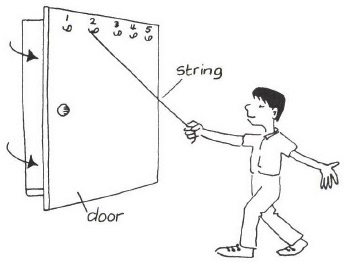
\includegraphics[width=0.4\textwidth]{./img/vso/doors-levers.jpg}
\end{center}

\begin{description*}
%\item[Subtopic:]{}
\item[Materials:]{Hooks/nails, string, door}
%\item[Setup:]{}
\item[Procedure:]{Place the hooks in the door 10-15 cm apart. Attach a string to the hooks, one at a time and try to pull the door open.}
%\item[Hazards:]{}
\item[Questions:]{Which hook makes it easiest to open the door?}
\item[Observations:]{The door is easier to open for hooks which are farther from the hinge.}
\item[Theory:]{Increasing the lever arm (distance from hinge) requires a smaller force to generate the moment needed to open the door. A short lever arm requires a larger force to achieve the same moment.}
%\item[Applications:]{}
%\item[Notes:]{}
\end{description*}

\subsection{Candle Balance}

\begin{center}
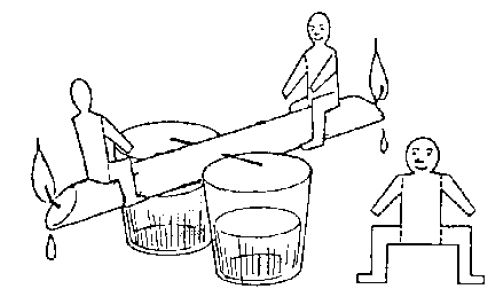
\includegraphics[width=0.45\textwidth]{./img/source/candle-balance.jpg}
\end{center}

\begin{description*}
%\item[Subtopic:]{}
\item[Materials:]{Candle, 2 cups, nail, paper}
\item[Setup:]{Cut out the paper figures as shown.}
\item[Procedure:]{Construct a candle balance as shown in the figure.}
%\item[Hazards:]{}
%\item[Questions:]{}
\item[Observations:]{The candle ends move up and down like a see-saw.}
\item[Theory:]{The candle ends lose drops of wax in
succession which causes a loss in weight at each
end.}
%\item[Applications:]{}
%\item[Notes:]{}
\end{description*}

\columnbreak

%==================================================================================================%

\section*{Principle of Moments}


\subsection[Determining an Unknown Mass]{Determining an Unknown \hfill \\ Mass}
\textbf{*NECTA PRACTICAL*}

\begin{center}
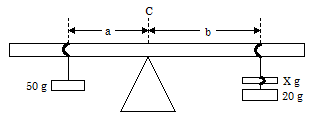
\includegraphics[width=0.49\textwidth]{./img/unknown-mass.png}
\end{center}

\begin{description*}
%\item[Subtopic:]{}
\item[Materials:]{Metre rule, triangular wooden block, string, dry cell, \nameref{sec:masses} (20 g and 50 g)}
%\item[Setup:]{}
\item[Procedure:]{Balance the metre rule on the wooden block (should be near 50 cm mark). Hang a 50 g mass a distance $a=5$ cm from the pivot point on one side. Balance the opposite side using a 20 g mass together with the dry cell. Record the length $b$ required to balance the ruler. Repeat for $a =$ 10 cm, 15 cm, 20 cm and 25 cm.}
%\item[Hazards:]{}
\item[Questions:]{Plot a graph of $a$ against $b$. Calculate the slope and use it to find the mass of the dry cell, $X$.}
%\item[Observations:]{}
\item[Theory:]{From the principle of moments, $(50 g)(a) = (20 + X g)(b)$. Canceling $g$ we find that $\frac{a}{b} = \frac{20 + X}{50} = \text{slope}$, so the value of $X$ can be determined.}
%\item[Applications:]{}
%\item[Notes:]{}
\end{description*}

\subsection{Mass of a Ruler}
\textbf{*NECTA PRACTICAL*}

\begin{center}
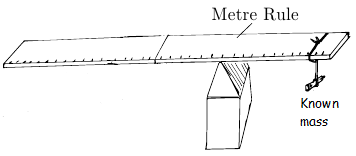
\includegraphics[width=0.45\textwidth]{./img/mass-of-ruler.png}
\end{center}

\begin{description*}
%\item[Subtopic:]{}
\item[Materials:]{Metre rule, triangular wooden block, \nameref{sec:masses}}
%\item[Setup:]{}
\item[Procedure:]{Place a known mass on one end of a metre rule. Adjust the position of the ruler until it balances on the knife edge.}
%\item[Hazards:]{}
\item[Questions:]{Determine the mass of the metre rule.}
%\item[Observations:]{}
\item[Theory:]{Using the known mass and measured distances on either side of the pivot, the unknown mass of the ruler can be found.}
%\item[Applications:]{}
%\item[Notes:]{}
\end{description*}

%==================================================================================================%

\section*{Centre of Gravity}


\subsection{Finding the CoG}

\begin{center}
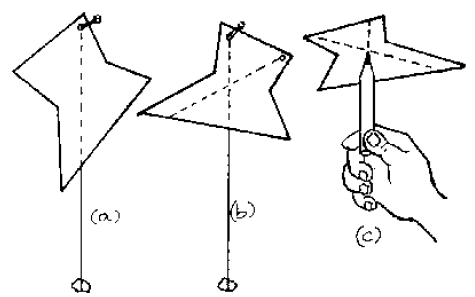
\includegraphics[width=0.4\textwidth]{./img/source/cog.png}
\end{center}

\begin{description*}
%\item[Subtopic:]{}
\item[Materials:]{Manila paper, pen, nail, sting, stone}
%\item[Setup:]{}
\item[Procedure:]{Cut a piece of manila paper into an odd shape. Suspend it from a nail and attach a string with a stone. Mark the position of the string at two points and then connect with a straight line using a ruler and pencil, as shown in (a). Repeat by fixing the nail in another point on the shape (b). Balance the shape at the point where the two lines meet.}
%\item[Hazards:]{}
%\item[Questions:]{}
\item[Observations:]{The shape balances at the intersection of the lines.}
\item[Theory:]{The intersection of the two lines locates the \emph{centre of gravity} of the object, and so it balances.}
%\item[Applications:]{}
%\item[Notes:]{}
\end{description*}

\subsection{CoG of a Ruler}

\begin{center}
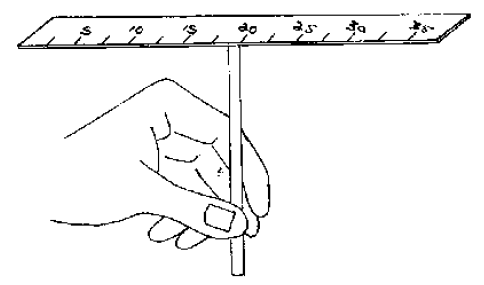
\includegraphics[width=0.4\textwidth]{./img/source/cog-ruler.png}
\end{center}

\begin{description*}
%\item[Subtopic:]{}
\item[Materials:]{Ruler, pencil/pen}
%\item[Setup:]{}
\item[Procedure:]{Find the centre of gravity of a ruler by balancing it on the tip of a pencil.}
%\item[Hazards:]{}
%\item[Questions:]{}
\item[Observations:]{The ruler balances at its center point.}
\item[Theory:]{The ruler's mass is evenly distributed. Thus, its centre of gravity acts at its geometrical centre.}
%\item[Applications:]{}
%\item[Notes:]{}
\end{description*}

%==================================================================================================%

\section*{Types of Equilibrium}

\begin{center}
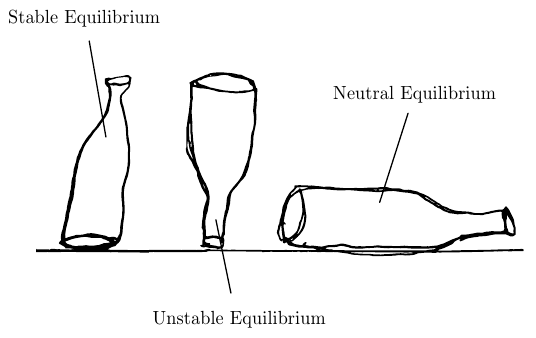
\includegraphics[width=0.49\textwidth]{./img/equilibrium.png}
\end{center}

A body is in \emph{stable equilibrium} if a small movement would rise its CoG, \emph{unstable equilibrium} if a small movement would lower its CoG, and \emph{neutral equilibrium} if a small movement would keep its CoG at the same level.

\subsection{Balancing Forks}

\begin{center}
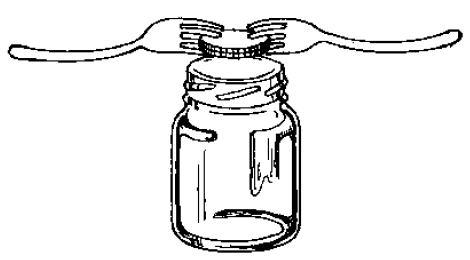
\includegraphics[width=0.45\textwidth]{./img/source/forks.png}
\end{center}

\begin{description*}
%\item[Subtopic:]{}
\item[Materials:]{2 forks, 2 coins, jar/can}
%\item[Setup:]{}
\item[Procedure:]{Take 2 coins and attach two forks as shown in the figure. Balance the arrangement on the edge of a jar or can.}
%\item[Hazards:]{}
%\item[Questions:]{}
%\item[Observations:]{}
\item[Theory:]{The CoG of the system is over the balancing surface, so it is in stable equilibrium.}
%\item[Applications:]{}
%\item[Notes:]{}
\end{description*}

\columnbreak

\subsection{Balancing Nails}

\begin{center}
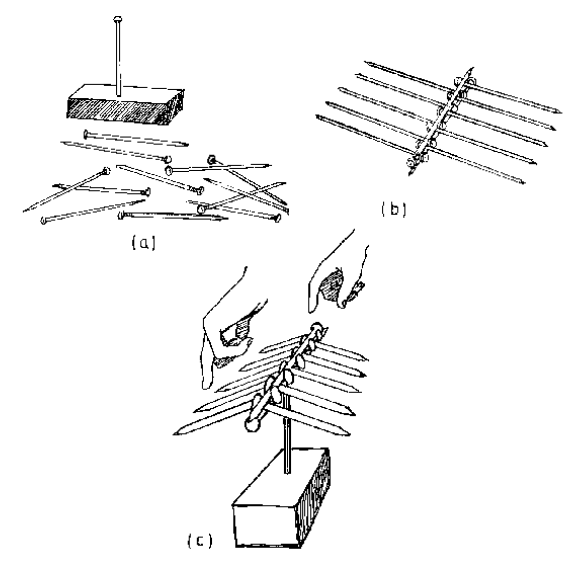
\includegraphics[width=0.45\textwidth]{./img/source/nails-1.png}
\end{center}

\begin{description*}
%\item[Subtopic:]{}
\item[Materials:]{Nails, piece of wood}
%\item[Setup:]{}
\item[Procedure:]{Stand one nail vertically in a piece of wood. Give students 10-12 nails and tell them to balance them all on top of this one nail.}
%\item[Hazards:]{}
%\item[Questions:]{}
\item[Observations:]{Arranging the nails according to figure (b), they can all be balanced.}
\item[Theory:]{The CoG is lower than the supporting head of the first nail, so the entire assembly is in \emph{stable equilibrium} and thus does not fall over.}
%\item[Applications:]{}
%\item[Notes:]{}
\end{description*}


\end{multicols}

\pagebreak